\section{Temperature measurement uncertainties}
The formula we use to retrieve the temperature is:
\begin{equation}
  \rm
  T_{by's} (F_{sun}, A_{eff}, \Delta P) = \frac{\frac{1}{2} F_{sun} A_{eff}}{10^{\frac{\Delta P}{10}} -1 }
\label{eq:tsys}
\end{equation}
Where $\rm  F_{sun}$ is  the sun flux  measured by  other observatory,
$\rm A_{eff}$ is the effective area in the sun's direction, $\Delta P$
is the power difference in dB (with 1dB = 50 ADC count) and the factor
$\rm \frac{1}{2}$ is  the polarization factor (we only  observe one of
the two polarizations). The uncertainties on $\rm T_{sys}$ is then:
\begin{equation}
  \rm       \sigma_{T_{sys}}^2      =      \frac{T_{sys}^2}{F_{sun}^2}
  \sigma_{F_{sun}}^2  + \frac{T_{sys}^2}{A_{eff}^2} \sigma_{A_{eff}}^2
  +   T_{sys}^2   \bigg(\frac{   \frac{\ln(10)}{10}   10^{\frac{\Delta
        P}{10}}}{10^{\frac{\Delta P}{10}}  - 1}\bigg)^2 \sigma_{\Delta
    P}^2
\end{equation}

\subsection{Sun flux uncertainties}
Here we check the precision we have on the sun flux. Up to now, we get
data  at \unit[2.8]{GHz}  (commonly called  f107) and  extrapolate the
value at  \unit[3.8]{GHz} with parameterisation  of the quiet  sun and
the slowly varying  sun. We can compare our  results with the Nobeyama
observatory data, which  collects data on the sun  flux at \unit[2 and
  4]{GHz} (we don't use their data yet because they don't release them
on the web). The figure~\ref{fig:sunflux} shows different fluxes: 

\begin{figure}[!ht]
 \centering
 \hspace*{-3ex}
 \subfigure{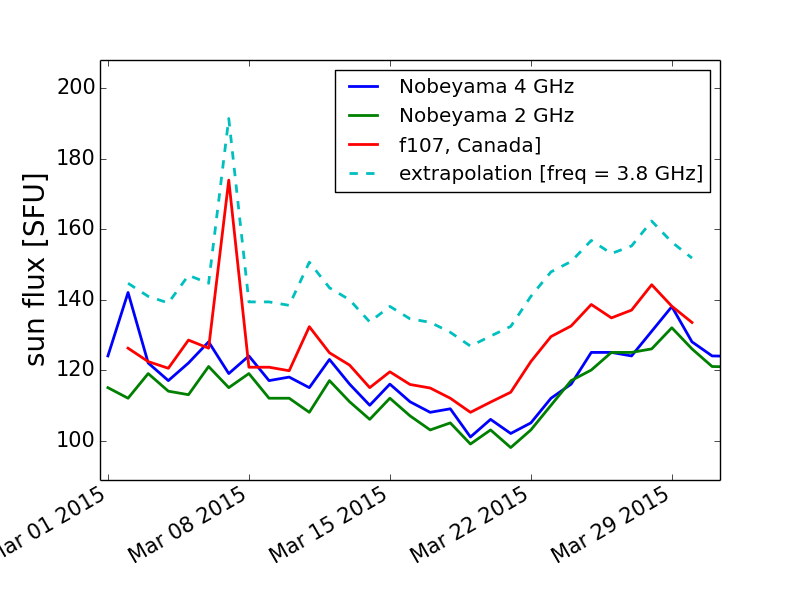
\includegraphics[width=0.49\linewidth]{sunfluxmarch.png}}
 \subfigure{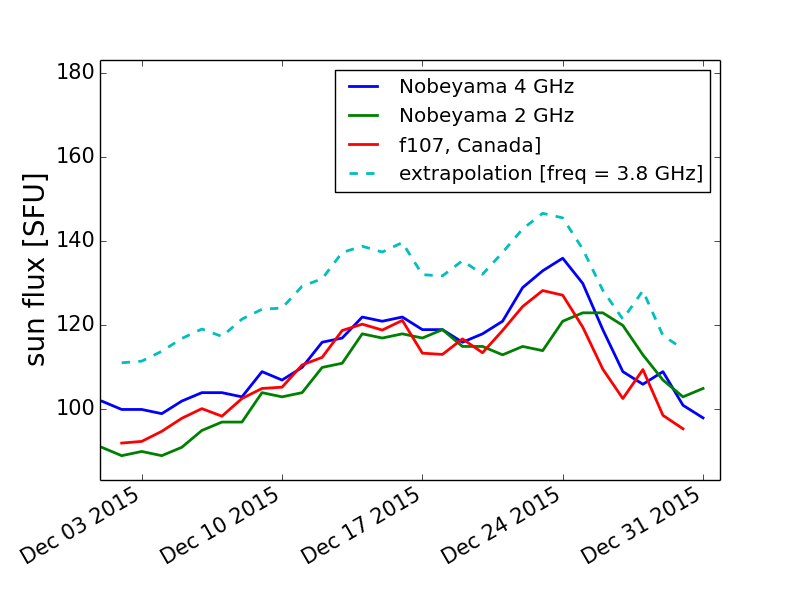
\includegraphics[width=0.49\linewidth]{sunfluxdec.png}}
%% \subfigure{\includegraphics[width=0.49\linewidth]{sunexpected.png}}
 \caption{sun flux for at different frequencies}
%%    Simulated  baseline  increase for  three  antennas  during the  sun
%%    passage.}
 \label{fig:sunflux}
\end{figure}
The value reported on the plots for the Nobeyama observatory are taken
from what is  displayed on their daily curves. I  don't really know if
this is an  average or the minimum value.  In any  case, the values at
\unit[2 and  4]{GHz} are lower than  what is measured  at the Canadian
site~\cite{sundata,  sundata2} by around  20\%. Since  I am  still not
sure of the meaning of the value for the Nobeyama data, I will account
for   an  uncertainty   of   20\%  in   the  temperature   calculation
(\textbf{this has to be improved either by taking the data of Nobeyama
  or by determining a precise uncertainty.}). 20\% corresponds also to
the precision given for the used parameterization~\cite{sunparam}.


\subsection{Effective area uncertainties}
Our measurement contains  an uncertainty on the effective  area, be it
because  of the  pointing direction  or our  limited knowledge  of the
gain.  We  only account  the possible shift  in zenith angle,  since a
shift in azimuth  would mainly affect the time  of maximum and slighly
the  amplitude of  the  signal.   We estimate  the  possible shift  in
pointing to  2$\rm ^{\circ}$.  The  resulting uncertainty on  the gain
depends   on   the   zenith   angle   at   the   sun   maximum.    The
Figure~\ref{fig:aeffuncert}  (left) shows  the antenna  effective area
and a  Gaussian fit as a  function of the zenith  angle. The resulting
uncertainties  on  the  effective   area  is  based  of  the  Gaussian
parameters   and    its   angle    dependence   is   shown    on   the
Figure~\ref{fig:aeffuncert} (right).
\begin{figure}[!ht]
 \centering
 \hspace*{-3ex}
 \subfigure{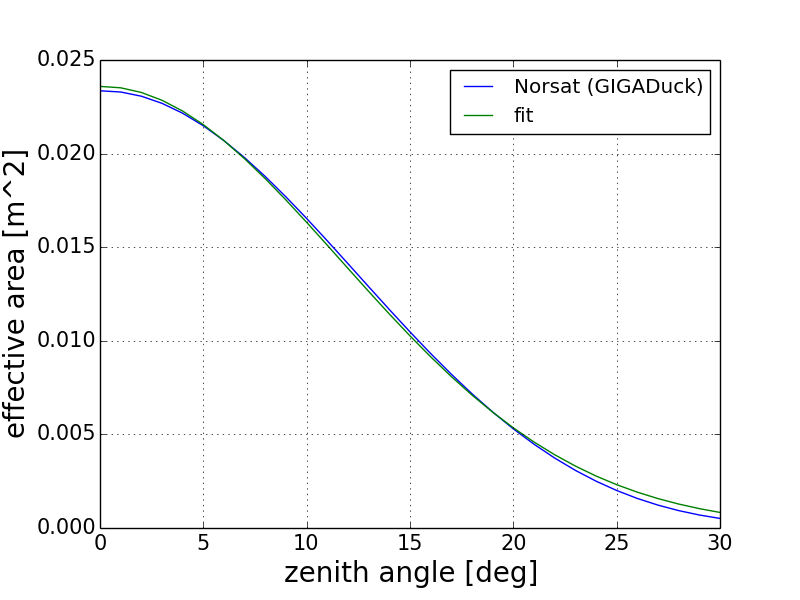
\includegraphics[width=0.49\linewidth]{aeff.png}}
 \subfigure{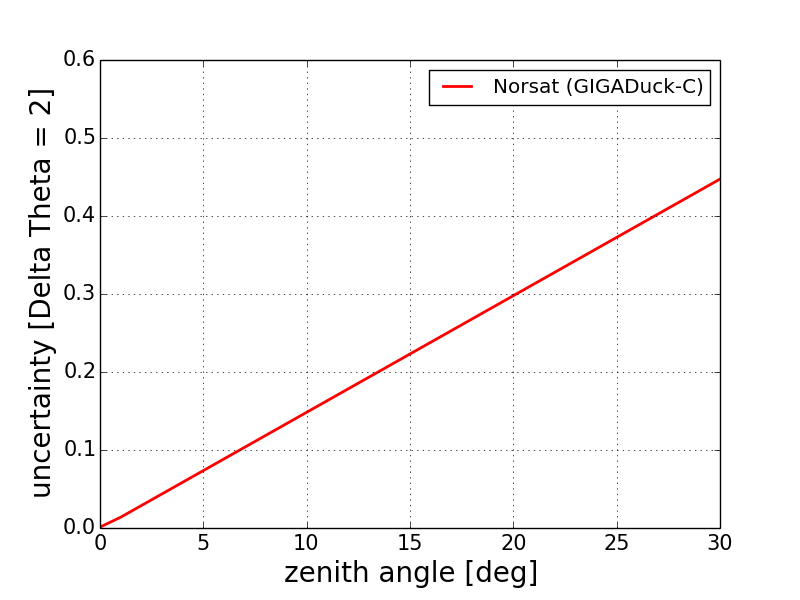
\includegraphics[width=0.49\linewidth]{sigmaaeff.png}}
 \caption{Effective  area of  the AInfo  antenna from  HFSS simulation
   (blue), Gaussian  fit (green).  Right: relative uncertainty  on the
   effective area}
 \label{fig:aeffuncert}
\end{figure}
We perform the  temperature measurement only during the  months when a
significant signal  from the  sun is expected,  that means when  it is
high in the  sky. The zenith angle at which the  sun signal is maximum
(in the simulation) is  shown in the figure~]\ref{fig:zenithofmax} for
  three antenna:  Vieira the  central detector that  points up  to the
  zenith, Chape  and Orteguina (see  figure~\ref{fig:sunsim} for their
  field of view).
\begin{figure}[!ht]
 \centering
 \hspace*{-3ex}
 \subfigure{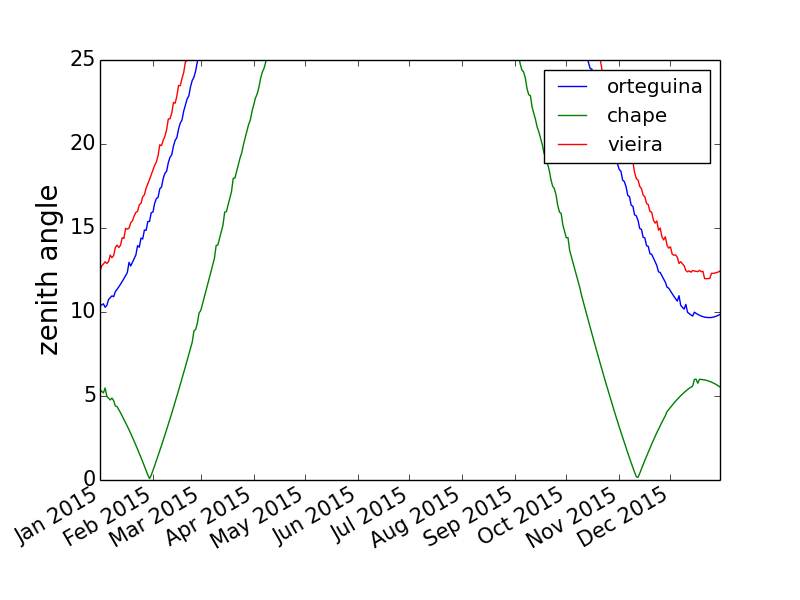
\includegraphics[width=0.49\linewidth]{zenithofmax.png}}
 \caption{Zenith angle when the sun signal is maximum as a function of
   the date}
 \label{fig:zenithofmax}
\end{figure}
The angle at  which the sun is observed when the  signal is maximum is
below  \unit[10]{$\rm  ^{\circ}$} for  Chape  but  around \unit[15  to
  20]{$\rm ^{\circ}$} in March for Vieira or Orteguina.


\subsection{Uncertainty on $\rm \Delta P$}
The uncertainty  on the measured power  induced by the  sun flux comes
from our  ability to measure a  variation of baseline on  an hour time
scale.   The  process  to   estimate  this  variation,  summed  up  in
section~\ref{sec:tempmeas}, is based  on a fit of the  sun bump with a
Gaussian function and the background with a second order polynominals.
There  aren't actually any  justification for  the background  fit. To
estimate the  error on  the $\rm  \Delta ADC$ we  make, we  change the
fitting   method    and   see    how   the   results    change.    The
figure~\ref{fig:fits}  shows the  results  of $\rm  \Delta  ADC$ as  a
function  of  the date  when  the baseline  is  either  fitted with  a
constant  and a  Gaussian  or with  a  second order  polynomial and  a
constant, on  the right side  is shown the corresponding  histogram of
the difference of the two methods. 
